\question{Câu 5}

Cho mạch khuếch đại tín hiệu được ghép liên tầng như hình vẽ. Trong đó, $Q_{1}$ là BJT có $\beta = 100$ và mã 2SC1815, và $Q_{2}$ có $\beta = 80$ có mã là 2N2907.

\begin{figure}[H]
	\centering
	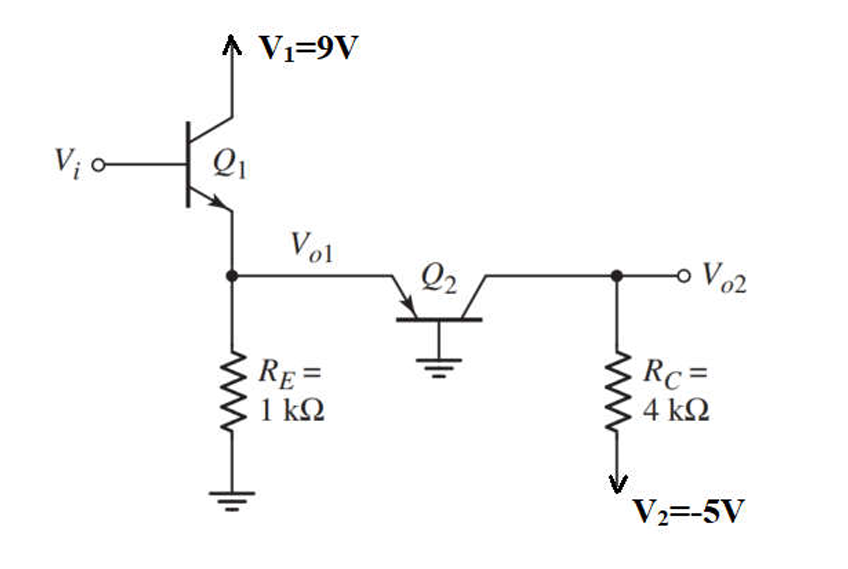
\includegraphics[width=.8\linewidth]{./my-chapters/my-images/Question5/debai.png}
\end{figure}

\answer{a}{Sử dụng phần mềm mô phỏng, vẽ VTC của mạch (ngõ vào $V_{i}$ và ngõ ra là $V_{o}$).}

Sử dụng chế độ DC Sweep trong Multisim để khảo sát VTC,

\begin{figure}[H]
	\centering
	\begin{minipage}{.5\linewidth}
		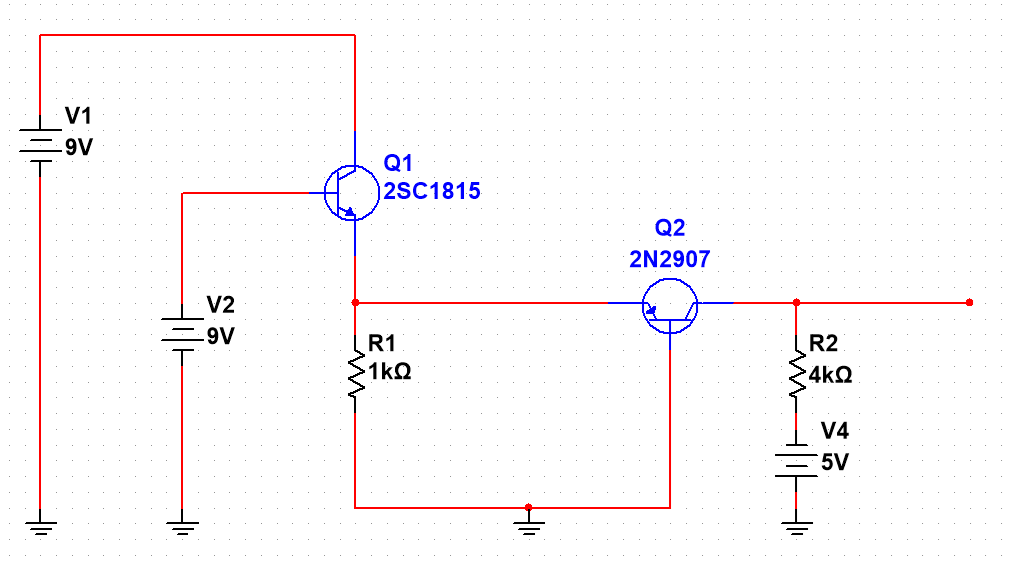
\includegraphics[width=.8\linewidth]{./my-chapters/my-images/Question5/a_mach.png}
	\end{minipage}
	\begin{minipage}{.4\linewidth}
		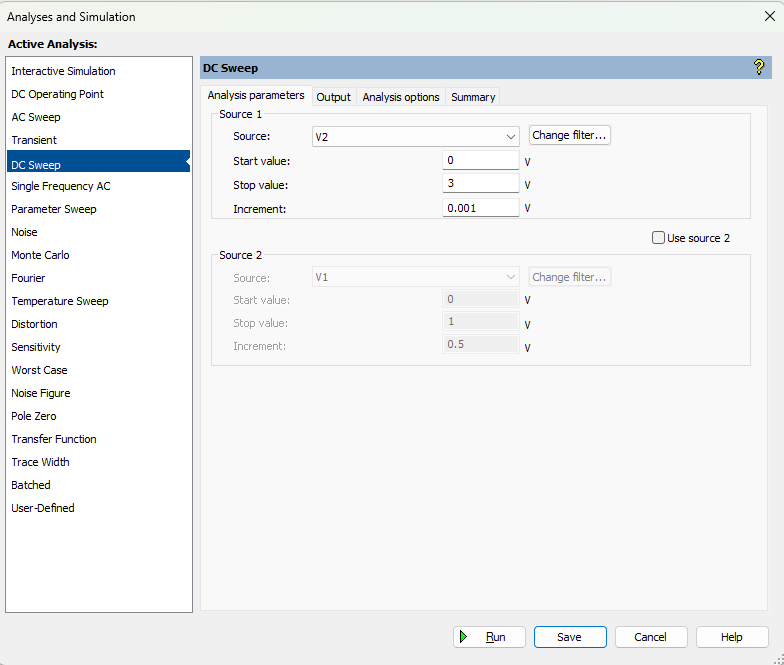
\includegraphics[width=.8\linewidth]{./my-chapters/my-images/Question5/a_dc_sweep.png}
	\end{minipage}
\end{figure}

\begin{figure}[H]
	\centering
	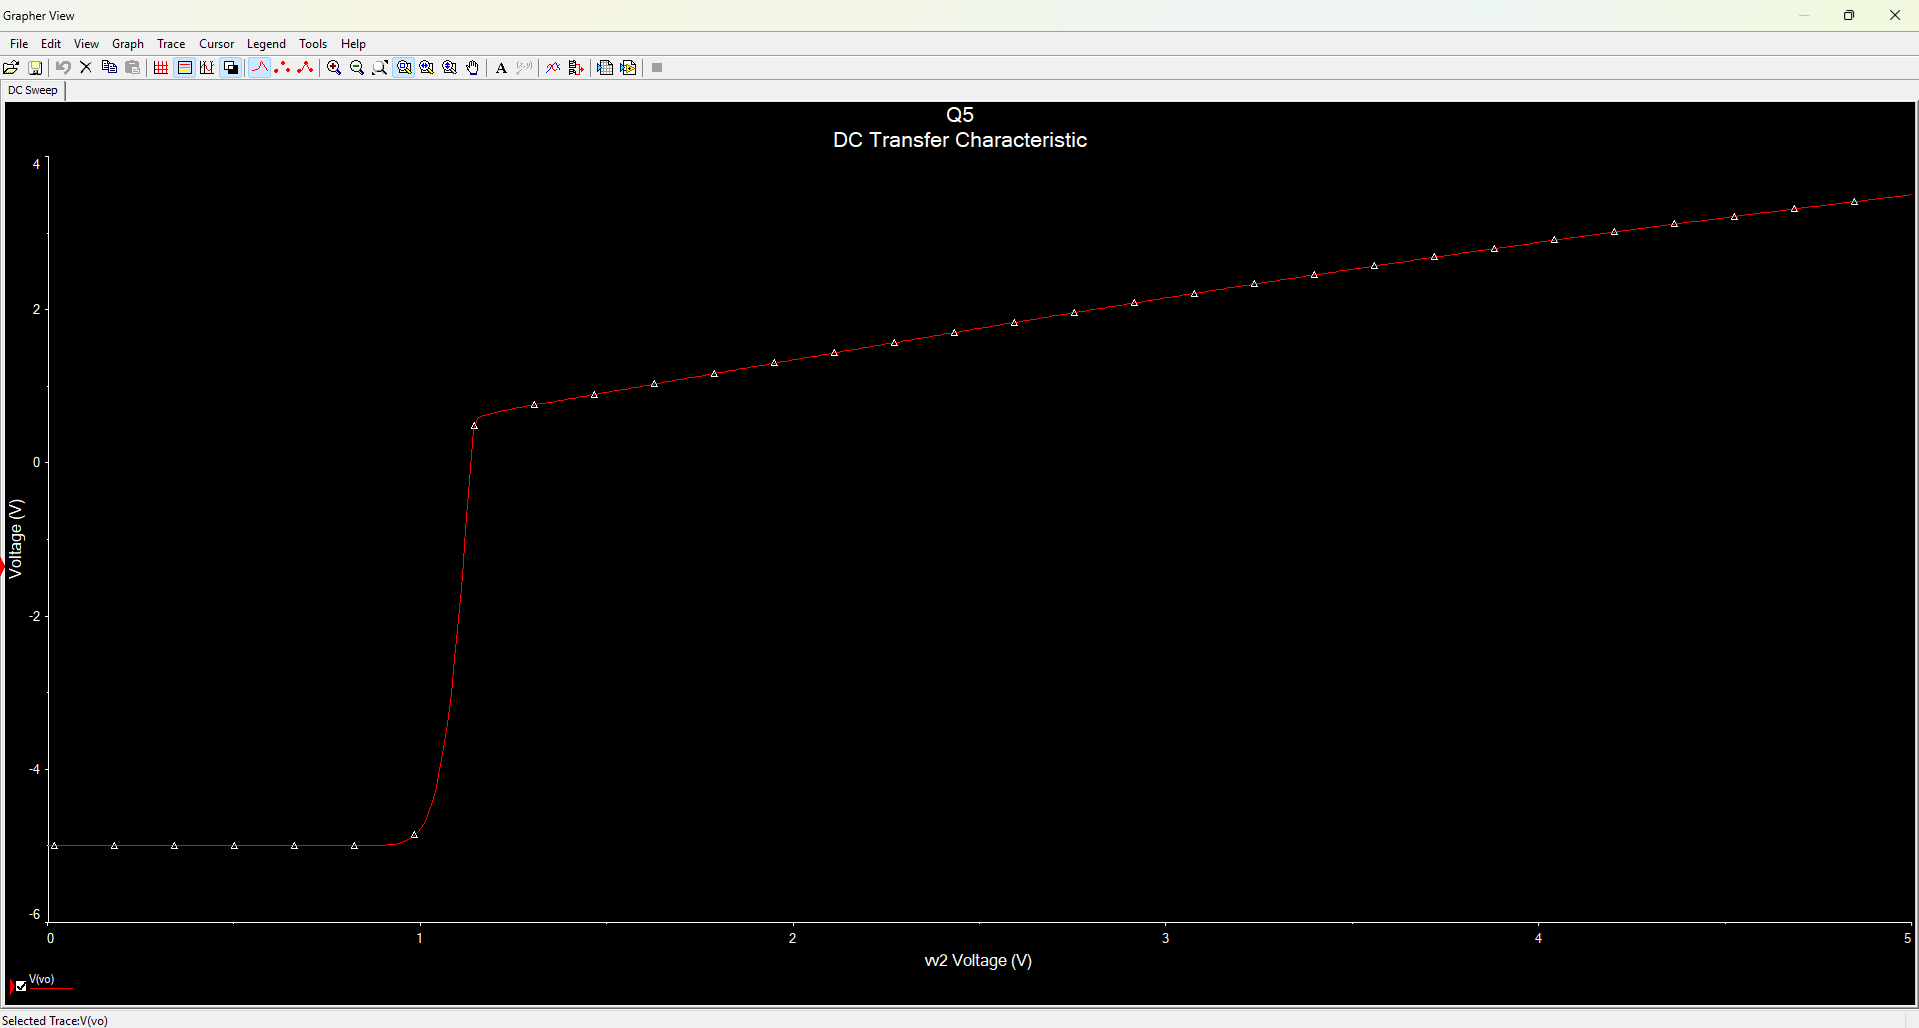
\includegraphics[width=.9\linewidth]{./my-chapters/my-images/Question5/a_VTC.png}
	\caption{VTC của mạch với ngõ vào $V_{i}$ và ngõ ra là $V_{o}$.}
\end{figure}

\answer{b}{Lựa chọn điểm phân cực của cả mạch trên VTC và thiết kế mạch ghép vào phía trước VTC để có được điểm phân cực đó.}

Quan sát VTC của mạch, để tín hiệu ngõ ra không bị méo dạng thì ta chọn điểm $Q$ với $V_{i} = 1.0998\,\text{V}$.

\begin{figure}[H]
	\centering
	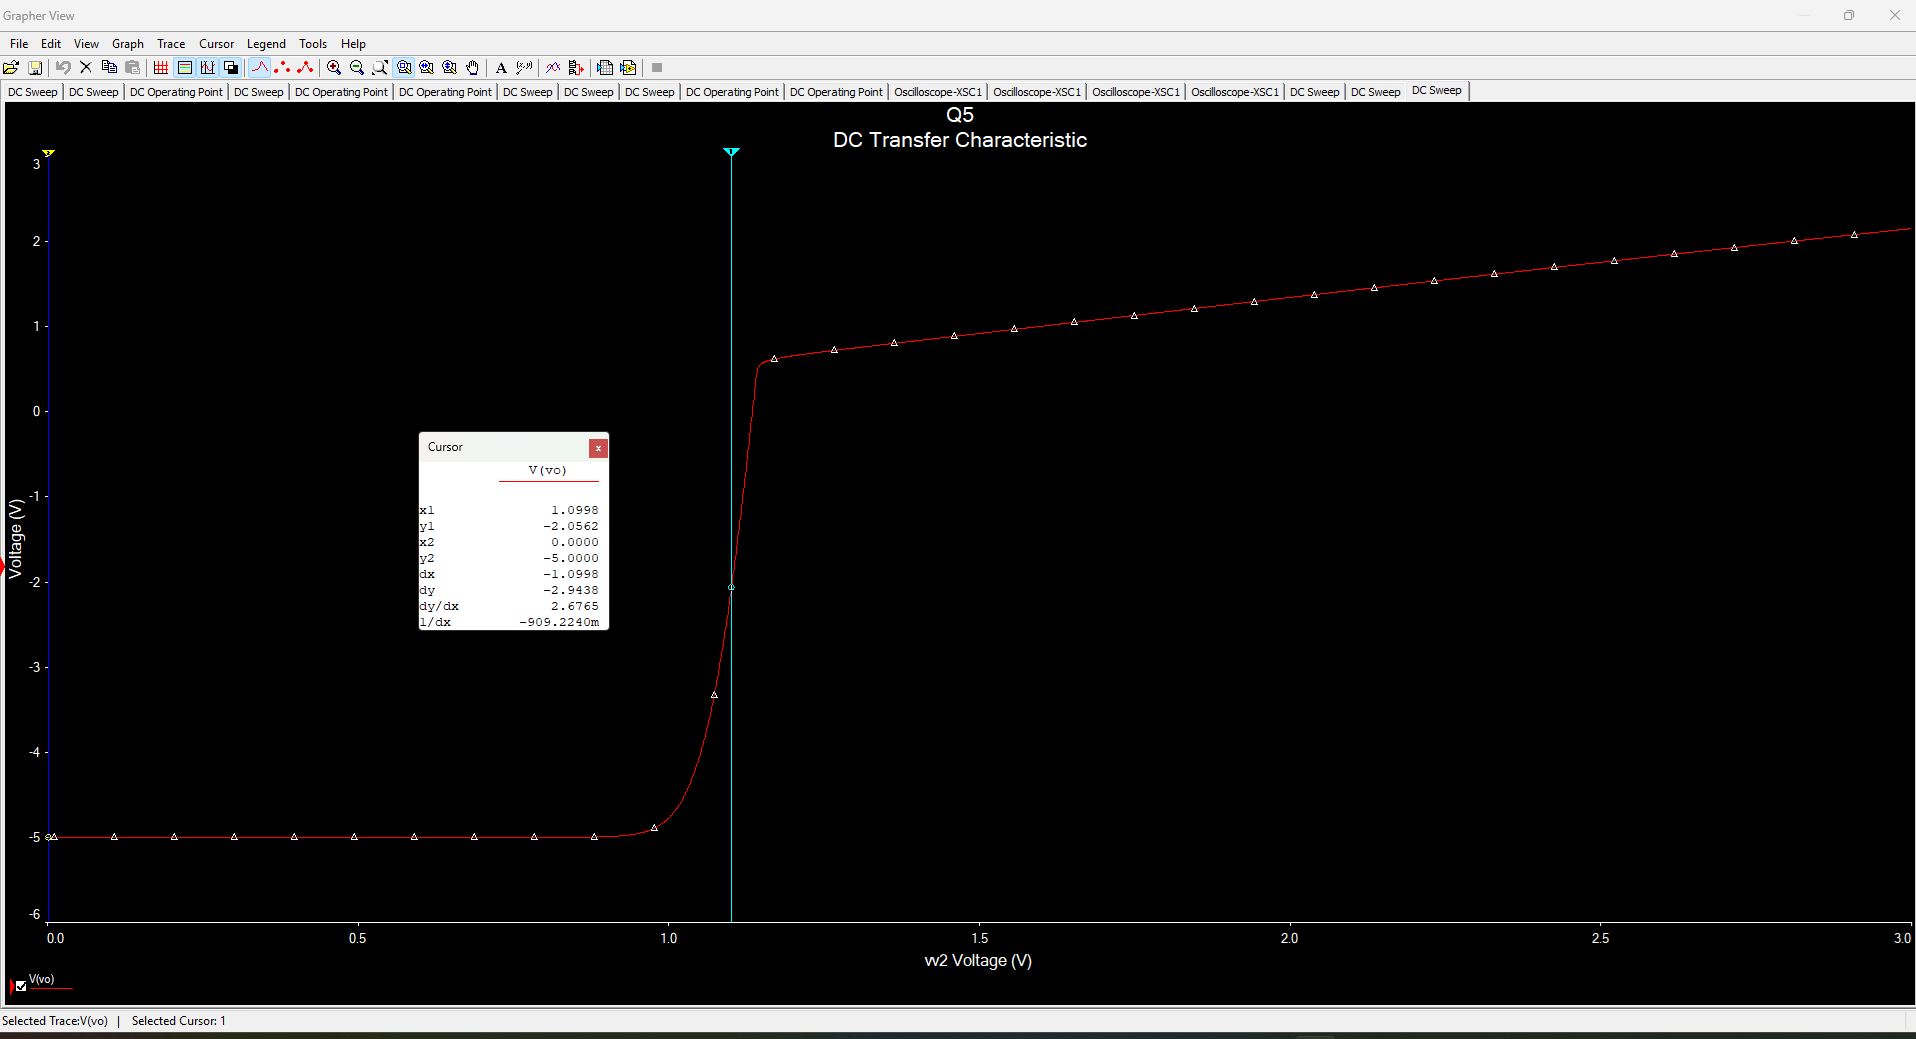
\includegraphics[width=.9\linewidth]{./my-chapters/my-images/Question5/b_Q_tong.png}
	\caption{Điểm hoạt động của toàn mạch rơi vào tầm $V_{i} = 1.0998\,\text{V}$ để tín hiệu $V_{o}$ không méo dạng.}
\end{figure}

Với $V_{i} = 1.0998\,\text{V}$, ta chọn được hai điểm:

\begin{figure}[H]
	\centering
%	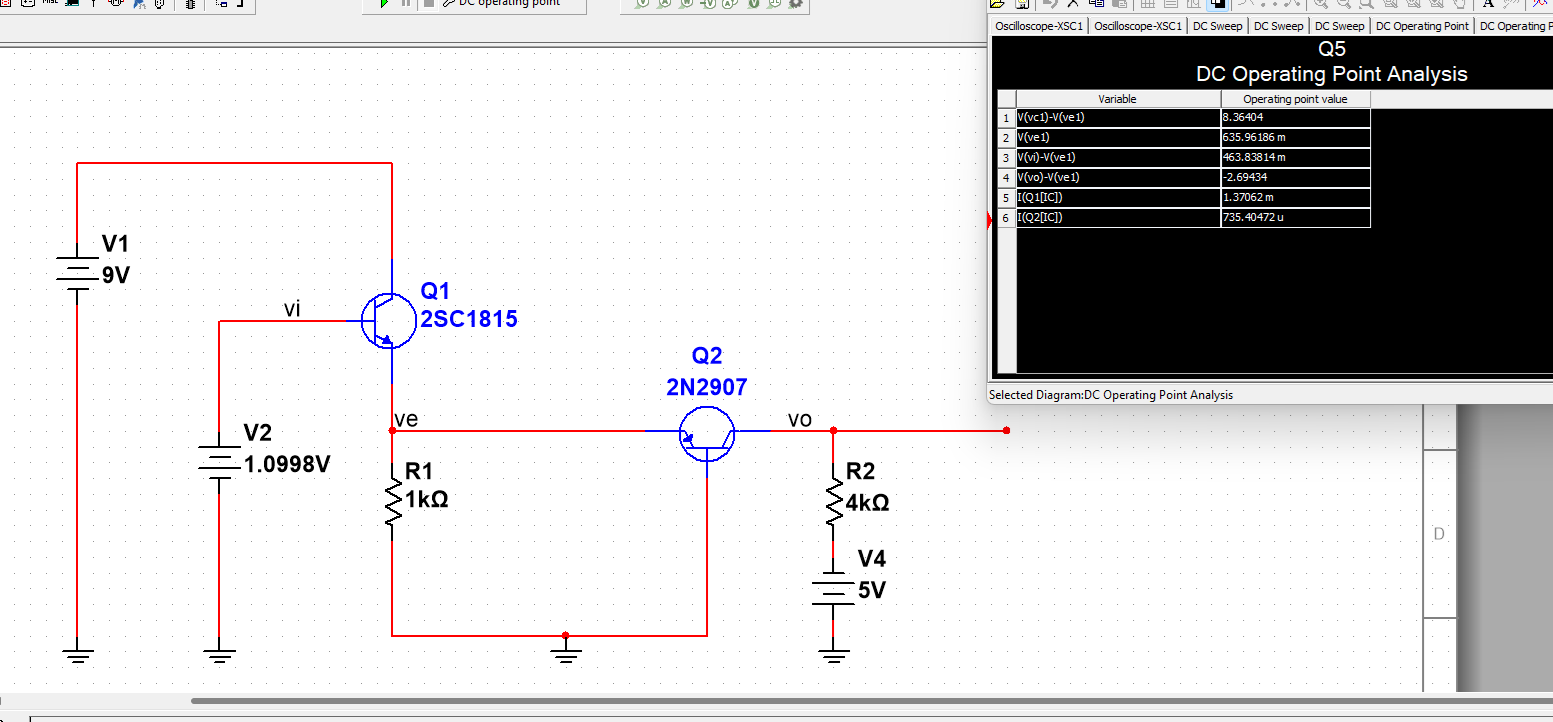
\includegraphics[width=.9\linewidth]{./my-chapters/my-images/Question5/b_Q_tung_mach.png}
	\begin{minipage}{.4\linewidth}
		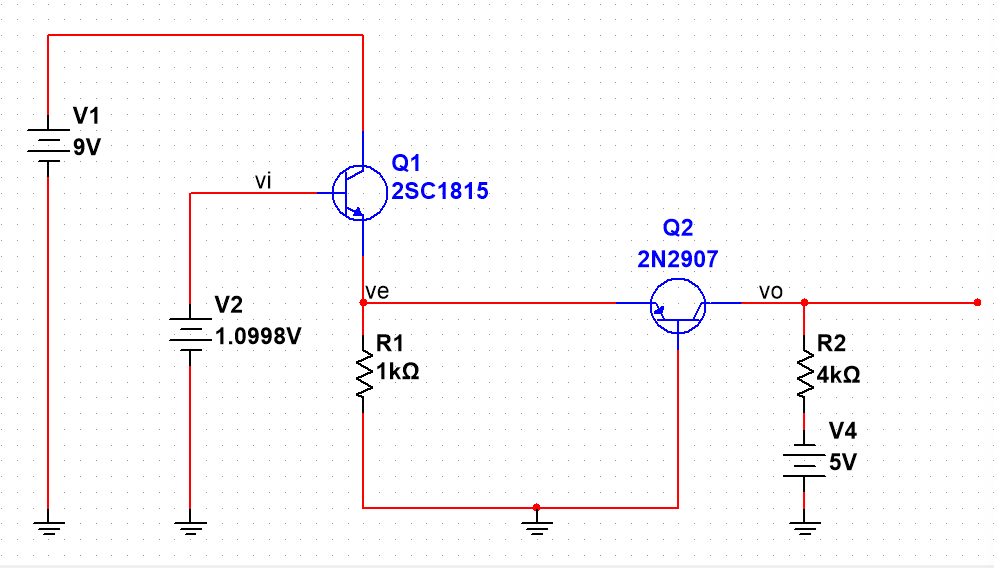
\includegraphics[width=\linewidth]{./my-chapters/my-images/Question5/b_Q_tong_hinh.png}
	\end{minipage}
	\begin{minipage}{.5\linewidth}
		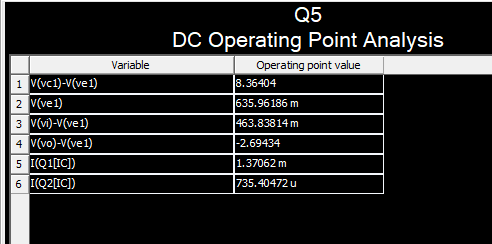
\includegraphics[width=\linewidth]{./my-chapters/my-images/Question5/b_Q_tong_bang.png}
	\end{minipage}
\end{figure}

\begin{itemize}[label=-, leftmargin=2cm]
	\item \finalresult{Q_{1} = (I_{CQ1}, V_{CEQ1}) = (1.3706\,\text{mA}, 8.3640\,\text{V})}
	\item \finalresult{Q_{2} = (I_{CQ2}, V_{CEQ2}) = (0.7354\,\text{mA}, -2.6943\,\text{V})}
\end{itemize}

